\chapter{Konzept}

Die Konzeption beschäftigt sich zunächst mit einem Überblick des ganzen Prozesses, von der Feature-Extraktion über die Komprimierung bis hin zur Gruppierung. Anschließend folgt eine nähere Betrachtung dieser drei wesentlichen Bestandteile und wie sie ineinandergreifen.\newline
Im Abschnitt \enquote{Feature Extraktion} werden die Feature-Deskriptoren vorgestellt, die hier verwendet werden: Zum einen der SIFT-Deskriptor, da dieser, neben guten praktischen Resultaten, bereits einigermaßen kompakt ist und auch direkt für die Komprimierung verwendet werden kann. Zum anderen wird ein Feature-Vektor konstruiert, der wesentlichen mehr Komponenten umfasst und sich somit für den Einsatz der Komprimierung eignet.\newline
Im folgenden Abschnitt \enquote{Autoencoder} wird auf der Basis der Arbeit von Zhao \cite{aed2016} ein Stacked Denoising Autoencoder eingeführt, der aus einem Feature-Vektor mit 3042 Komponenten, eine Darstellung des Features in einem Raum mit 36 Dimensionen lernt.\newline
Im letzten Abschnitt wird das Bag of Visual Words Modell näher betrachtet: Es werden auf Basis der Analyse parallele Varianten des Clustering- und Histogramm-Algorithmus entworfen, die sich zur Ausführung auf Grafikkarten eignen, die CUDA unterstützen. Abschließend wird behandelt, wie der Bag of Visual Words verwendet werden kann, um ein Modell zu generieren bzw. die Ähnlichkeit zweier Bilder zu bewerten.

\section{Modell}

In der Analyse wurden die wesentlichen Bestandteile identifiziert, welche hier zur Gruppierung von Bildern dienen sollen. Um dies zu erreichen wird ein dreistufiges Modell vorgeschlagen, dass in Abbildung \ref{img:model} skizziert ist. Jede \enquote{Zeile} entspricht hier einer Phase der Verarbeitung. Die Ein- bzw. Ausgaben sind mit durch die Farbe grün gekennzeichnet, die Schritte zur Datenverarbeitung durch Orange. Diese Phasen werden im Folgenden detailliert dargestellt, hier soll jedoch zuerst ein Überblick über den Ablauf gegeben werden. Die drei Phasen zum Erzeugen eines Modells laufen wie folgt ab:\newline 

\begin{itemize}
	\item \textbf{Extraktion} Zuerst muss das Verfahren bestimmt werden, mit denen die Features gewonnen werden sollen. Je nach Anwendungsfall sollte dieses Verfahren austauschbar sein. Zu Beginn werden aus den Bilddaten \textit{Images} durch einen Feature-Extraktor die Feature-Vektoren \textit{Features A} erhoben. Bei den Bilddaten handelt es sich um eine Liste von Matritzen, welche die Intensitätswerte von Bildpixeln kodiert. \textit{Features A} ist ein Vektor von Features, die abhängig vom Verfahren verschiedene Eigenschaften beschreiben.
	\item \textbf{Komprimierung} Um die Komponenten in einem Feature-Vektor auf die Wesentlichen zu reduzieren, erfolgt eine Komprimierung durch einen Autoencoder. Die Phase des Autoencoders ist hierbei optional und daher gestrichelt dargestellt. Sollten die Features nicht durch den Autoencoder komprimiert werden, so ist der Vektor \textit{Features B} gleich dem Vektor \textit{Features A}. Andernfalls enthält \textit{Features B} die komprimierten Features.
	\item \textbf{Gruppierung} In der dritten Phase nimmt der Bag of Visual Words die Features aus der vorigen Phase entgegen und generiert hieraus das \textit{Codebook}. Da die \textit{Visual Words} des \textit{Codebooks} den erzeugten Clustern entsprechen, ist das Codebook selbst eine Liste von Clustern. Die Cluster wiederum sind Stellvertreter einer Menge von Features, daher sind sie ebenfalls ein Vektor mit der gleichen Anzahl an Komponenten wie die Features in \textit{Features B}.
\end{itemize} 

\begin{figure}
	\centering
	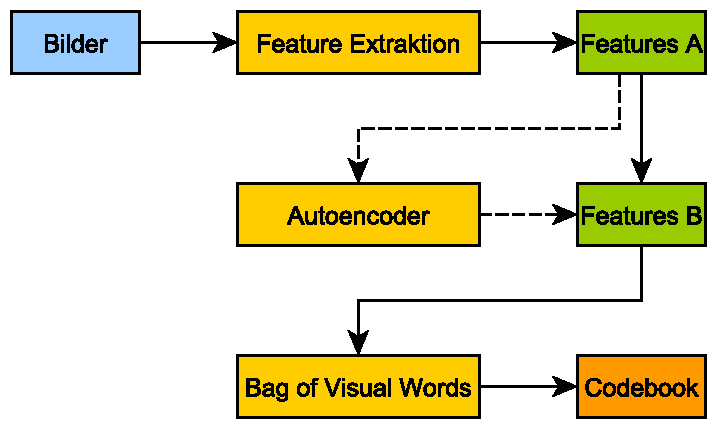
\includegraphics[scale=0.85]{images/model.pdf}
	\caption{Aufbau des Modells}
	\label{img:model}
\end{figure}

Das Erzeugen der \textit{Visual Words} aus einem Bild läuft in den ersten beiden Schritten analog ab, nur das die Menge \textit{Images} aus genau einem Bild, dem zu verarbeitenden, besteht. Die Features werden erst extrahiert und dann optional komprimiert. Für diese Schritte müssen auch exakt die gleichen Parameter verwendet werden, d.h.:

\begin{itemize}
	\item Der gleiche Feature-Detektor bzw. -Deskriptor muss gewählt werden.
	\item Eine Komprimierung muss stattfinden, wenn dies im Training der Fall war. Andernfalls darf sie nicht erfolgen.
	\item Das gleiche Netzwerk zur Erzeugung der komprimierten Features muss gewählt werden.
\end{itemize}

In der dritten Phase verwendet der Bag of Visual Words das vorher generierte \textit{Codebook} und die Features aus der vorigen Phase, um die \textit{Visual Words} zu ermitteln.

\section{Feature Extraktion}

Da es zahlreiche Verfahren zur Detektion und Extraktion von Features aus Bildern in Literatur und Praxis gibt, können diese unmöglich alle gleichermaßen Beachtung finden. In der Analyse wurde daher beschlossen, zunächst ein Clustering der Bilder anhand einer Objekterkennung zu realisieren. Um den Prozess des Clusterings zu beschleunigen, soll der Feature-Vektor kompakt sein. Eine solche Kompression kann durch einen Autoencoder erreicht werden. Die Effektivität hängt hierbei stark von den verwendeten Daten ab. Die Vektoren sollten initial möglichst viele Komponenten umfassen, um ein tiefes Netz konstruieren zu können. Ein solcher Deskriptor muss aber eigens für den Autoencoder trainiert werden: Die meisten etablierten Deskriptoren ermöglichen eben nicht die Konstruktion eines tiefen Netzes. Die Verwendung eines alternativen Deskriptors ist daher aus zwei Gründen plausibel:

\begin{itemize}
	\item Da die Schritte im Prozess aufeinander aufbauen, hängt die Qualität der Ergebnisse des Bag of Visual Word Verfahrens auch vom Autoencoder ab. Um den Bag of Visual Words an sich testen zu können, soll ein bereits kompakter, praktisch bewährter Deskriptor als Alternative dienen.
	\item Es ist denkbar, dass der Schritt der Komprimierung nicht in allen Fällen notwendig bzw. sinnvoll ist, da der Deskriptor bereits kompakt genug ist.
\end{itemize} 

Der von Zhao \cite{aed2016} entwickelte Autoencoder nimmt daher einen eigens kreierten Feature-Vektor als Eingabe entgegen. Die \textit{keypoints} werden hier durch den Difference of Gaussians ermittelt. Um jeden der \textit{keypoints} wird eine Nachbarschaft der Größe $41 \times 41$ betrachtet. Von diesen Ausschnitten werden die Gradienten in horizontale und vertikale Richtung bestimmt. Bei einem Einsatz eines Gaußfilters mit einer Filterkerngröße von $3 \times 3$, ergeben sich somit pro Richtung $1521$ Werte, die den Ausschnitt beschreiben. Der resultierende Feature-Vektor besitzt somit, für beide Richtungen, insgesamt $3042$ Komponenten.\newline
Um das Clustering-Verfahren auch ohne einen Autoencoder anwenden zu können, bzw. sicherzustellen, dass andere Feature-Deskriptoren für Bilder direkt verwendet werden können, soll in einem Test auch SIFT Gegenstand sein. So kann nicht nur die Qualität der Ergebnisse der beiden Deskriptoren verglichen werden, sondern auch Auswirkungen auf die Laufzeit des Bag of Visual Words.

\section{Autoencoder}

In diesem Ansatz wird ein Stacked Denoising Autoencoder zur Komprimierung eines Feature-Vektors entworfen, wie er in der Arbeit von Zhao \cite{aed2016} vorgeschlagen wurde. Hierfür wird zunächst im Abschnitt \enquote{Modell} ein objektorientiertes Modell entworfen, dass den Autoencoder, wie er in der Analyse beschrieben wurde, abbildet. Durch dieses Klassenstruktur lassen sich nun beliebige Autoencoder definieren. Im Teil \enquote{Parameter} wird dann auf den konkreten Autoencoder eingegangen, den Zhao entworfen hat.

\subsection{Entwurf des Modells}

Im Klassendiagramm in Abbildung \ref{img:ae_class} sind die wesentlichen Bestandteile eines Autoencoders erfasst: Der Großteil der Parameter sind private Variablen, die bei Erzeugung, also im Konstruktor, übergeben werden müssen. Die Anzahl der Schichten ergibt sich durch die Anzahl der Elemente in \textit{layers}. Jede Ganzzahl steht hier für die Anzahl der Neuronen in einer Schicht. Die Gewichte zwischen zwei Schichten sind in \textit{weights} gespeichert. Ein  Gewicht $w_{ij}$ von Neuron $i$ zu Neuron $j$ zwischen zwei Schichten befindet sich an der Position \textit{weights[i][j]}. Da zwischen Schichten unterschiedliche Aktivierungsfunktionen verwendet werden können, wird eine Liste  mit einer Aktivierungsfunktion pro Schichtpaar erwartet. \newline
Durch \textit{encode} wird der Autoencoder genutzt, um die Testdaten zu komprimieren. Die Anzahl der Koordinaten eines Features muss hier gleich der Anzahl der Neuronen in der ersten Schicht des Autoencoders sein. Die Methode \textit{decode} kehrt den Prozess der Enkodierung wieder um. Hier werden entsprechend Features erwartet, die genauso viele Koordinaten wie die letzte Schicht des Netzwerks aufweisen.
  
\begin{figure}
	\centering
	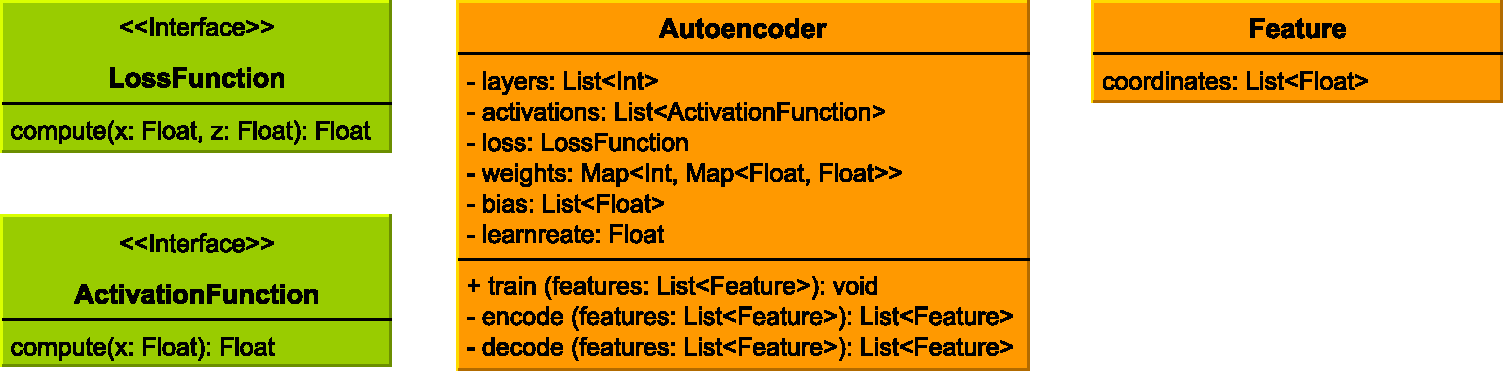
\includegraphics[scale=0.6]{images/ae_class.pdf}
	\caption{Klassendiagramm des Autoencoders}
	\label{img:ae_class}
\end{figure}

\subsection{Parameter des Netzes}

Nachdem nun eine Struktur geschaffen wurde, in der sich beliebige Autoencoder definieren lassen, soll das von Zhao vorgeschlagene Netzwerk näher betrachtet werden. Die Leistung dieses Autoencoders wurden unter verschiedenen Kriterien mit denen der Hauptkomponentenanalyse (PCA) und SIFT-PCA verglichen. Dabei erkannte der Autoencoder in fast allen die gleichen Features, jedoch durch einen 36 statt 128-elementigen Feature-Vektor. Der Encoder des vorgeschlagenen Modells besteht aus fünf Schichten, deren Neuronenanzahl sukzessive reduziert wird, bis schließlich die kleinste Schicht mit 36 Neuronen erreicht wird. Abbildung \ref{img:ae_model} zeigt die Schichten des Encoders sowie Decoders. Der Decoder ist umgekehrt aufgebaut und auch die Gewichte der Kanten zwischen zwei Neuronen entsprechen ihren Pendants im Encoder.

\begin{figure}
	\centering
	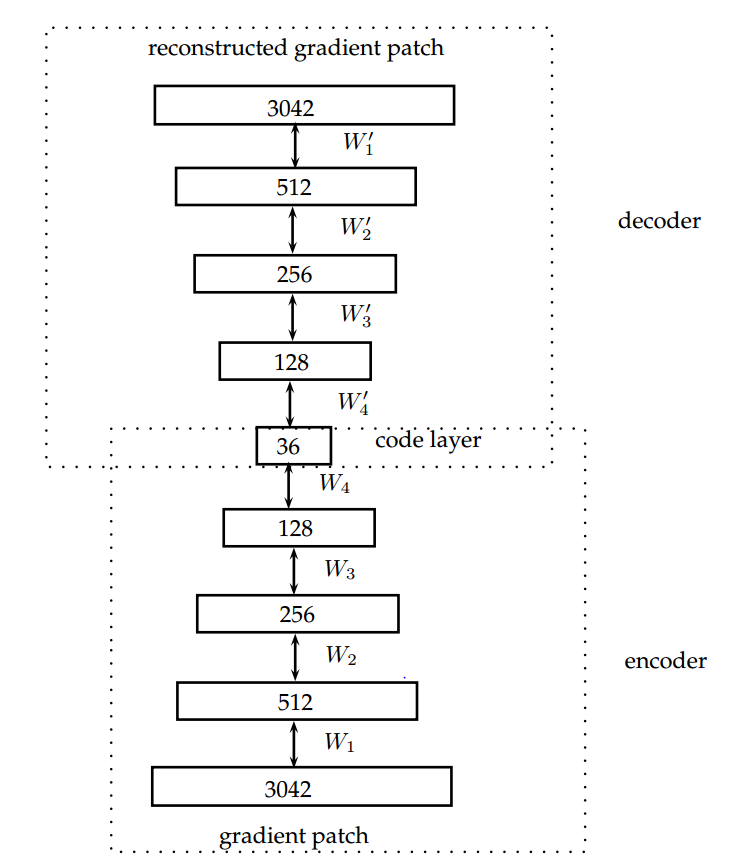
\includegraphics[scale=0.6]{images/ae_model.png}
	\caption{Schichten des verwendeten Autoencoders \cite{aed2016}}
	\label{img:ae_model}
\end{figure}

Die Hyperparameter für das verwendete Modell sind vollständig dokumentiert. Dabei wird zwischen dem \textit{Pretraining} und dem \textit{Finetuning} unterschieden: Zunächst findet das \textit{Pretraining} statt, also das trainieren der einzelnen Enkoder-Paare. Jedes Paar wird für 500 Iterationen trainiert und die Lernrate auf $0.05$ gesetzt. Beim \textit{Finetuning} wird dann das Backpropagation-Verfahren angewendet. Das ganze Netz wird für 700 Iterationen mit einer Lernrate von $0.03$ trainiert. Zhao verwendete hier für die Lernrate einen Wert von $2\%$, sodass $l = 0.02$. Als Aktivierungsfunktion wird in beiden Phasen die logistische (sigmoid) Funktion verwendet und ein \textit{batch} enthält 100 Elemente. Das Netz sieht so in einem \textit{foward} und \textit{backward pass} je 100 Trainingsexemplare. Da dies im Wesentlichen die Laufzeit durch eine Verwendung von mehr Speicher bewirkt, kann diese Zahl bei ungenügenden Ressourcen auch reduziert werden. Sowohl beim \textit{Pretraining} als auch beim \textit{Finetuning} werden 30\% der Eingabe korrumpiert.

\section{Bag of Visual Words}

In der Analyse wurde bereits eine sequentielle Varianten von Lloyds-Algorithmus und ein sequentieller Histogramm-Algorithmus vorgestellt und aufgezeigt, an welchen Stellen eine Parallelisierung der Berechnung durch Grafikkarten erfolgen kann. Im Folgenden wird aus diesen Informationen je Algorithmus eine parallele Version abgeleitet, welche sich für die Realisierung als CUDA Programm eignen.
Im Abschnitt Modell wird dann der Aufbau des Modells und Ablauf der Funktionsaufrufe skizziert. Zur Interaktion stehen einem Anwender im Wesentlichen eine Funktion zu Generierung eines Modells und zur Berechnung der \textit{Visual Words} eines Bildes zur Verfügung.

\subsection{Paralellisierung von Llyods Algorithmus}

Nachdem in der Analyse bereits anhand einer sequentiellen Variante von Lloyds Algorithmus, die zu parallelisierenden Berechnungen identifiziert wurden, wird hier der Ablauf einer parallelen Version vorgestellt. Das nachfolgende Listing aus der Arbeit von Zechner und Granitzer \cite{akc2009} illustriert den Ablauf solch eines Algorithmus in Pseudocode. Die Funktion \textit{lloyd\textunderscore gpu} erwartet als Parameter die zu quantisierenden Vektoren $V$ und eine initial leere Liste der Cluster $C$. Der Thread in einem Block mit der \textit{threadId} 0 fungiert hier als Master für die anderen Threads. Die Initialisierung der Cluster mit zufälligen Vektoren aus $V$ wird ebenfalls von diesem übernommen. Die Zuweisung von Vektoren zu Clustern kann parallelisiert werden, in dem pro Feature-Vektor ein Thread verwendet wird: Jeder Thread berechnet für seine Feature-Vektoren die Distanz zu allen Clusterschwerpunkten. Der Index des Clusters, der am Nächsten ist, wird in einer Liste $l$ \textit{(labels)} unter dem Index des Vektors gespeichert. Dieser Prozess ist in Pseudocode in Zeile 6 und 7 ausgedrückt. Bevor die Cluster aktualisiert werden, müssen die Threads synchronisiert werden: Andernfalls ist nicht garantiert, dass die Berechnung jedes Threads abgeschlossen ist. In Zeile 11 übernimmt der Master-Thread die Neuberechnung der Clusterschwerpunkte. In Zeile 13 werden die Vektoren in den jeweiligen Clusterschwerpunkt mitaufgenommen (aufsummiert). In Zeile 14 wird $m$ \textit{members}, die Anzahl der Vektoren pro Cluster, für jeden neuen Vektor inkrementiert. In Zeile 15 und 16 erfolgt dann die Berechnung des Durchschnitts aller Clusterschwerpunkte.

\begin{figure}
\begin{lstlisting}[mathescape=true, style=Math]
lloyd_gpu(V, C, k)
	if threadId == 0
		$c_j = rand(v_i) \in V, \: j = 1,...,k, \: c_j \neq c_i \: \forall i \neq j$
	synchthreads
	
	until convergence
		for each $v_i \in V_{threadId}$
			$l_i = \arg \min D(c_j, v_i)$
		synchthreads
		
		if threadId == 0
			for each $v_{i} \in V$
				$c_{l_i} = c_{l_i} + v_i$
				$m_{l_i} = m_{l_i} + 1$
			for each $c_j \in C$
				$c_j = \frac{1}{m_j} c_j$
\end{lstlisting}
\caption{Ablauf der parallelen Variante von Lloyds Algorithmus \cite{akc2009}. }
\end{figure}

\subsection{Parallele Reduzierung von Histogrammen}

Die Berechnung eines Histogramms kann parallelisiert werden, da die Operation assoziativ und kommutativ ist: Es spielt keine Rolle, in welcher Reihenfolge die Daten abgearbeitet werden bzw. in welcher Reihenfolge die Klassen inkrementiert werden. Wenn das zu beschreibende Histogramm im \textit{global memory} vorliegt, wird die Berechnungsgeschwindigkeit stark reduziert, da viele Threads auf die gleichen Speicheradressen des Histogramms schreibend zugreifen. Damit es nicht zu Lese- / Schreibanomalien kommt, muss das Inkrementieren einer Klasse atomar sein, d.h. zwischen Lese- und Schreibzugriff darf kein anderer Thread auf die Adresse zugreifen. Dies wird in CUDA durch die Operation \textit{atomicAdd} realisiert. Damit die Anzahl an Threads, die auf dieselbe Adresse schreiben eingeschränkt wird, arbeitet jeder Block auf einem lokalen Histogramm im \textit{shared memory}. Wenn alle Blöcke ihre lokalen Histogramme berechnet haben, müssen diese noch in das Histogramm im \textit{global memory} kumuliert werden.\newline
In nachfolgendem Listing ist solch ein Histogrammalgorithmus unter CUDA aufgeführt. Als Parameter werden hier die Features \textit{features}, die Cluster \textit{clusters}, das zu beschreibende Histogramm \textit{histo}, die Anzahl an Komponenten in einem Feature \textit{featureSize}, die Anzahl der Features \textit{count} sowie die Anzahl der Cluster \textit{k} erwartet. Zunächst wird in Zeile 3 und 4 der nötige \textit{shared memory} allokiert. Das Schlüsselwort \textit{extern} gibt an, dass die Größe des \textit{shared memory} bei Aufruf des \textit{kernels} mitgegeben wird (in den dreifachen, spitzen Klammern). Die Klassen des privaten Histogramms werden alle mit 0 initialisiert und die Threads synchronisiert. In Zeile 11 wird der Index des ersten Features berechnet, dessen Cluster dieser Thread berechnen soll. Die Anzahl der Features die der Block insgesamt berechnet ergibt sich dann aus der Block- und Griddimension. Die \textit{while}-Schleife in Zeile 14 wird dann für all diese Features durchlaufen. Hier wird der Index des nächsten Clusters berechnet und die entsprechende Klasse des privaten Histogramms inkrementiert. Da nicht jeder Block unbedingt gleich viele Features bearbeitet, also wenn die Anzahl der Features nicht ein Vielfaches der Blockdimension ist, müssen die Threads nach der Schleife wieder synchronisiert werden. Abschließend werden die Werte des privaten Histogramms eines Blocks in das globale kopiert.

\begin{lstlisting}[style=CUDA]
__global__
void histogram_kernel (float *features, float *clusters, unsigned int *histo, int featureSize, int count, int k) {
	extern __shared__ int *sharedMemory[];
	unsigned int histo_private = (unsigned int*) sharedMemory;
	
	if (threadIdx.x < k) {
		histo_private[threadIdx.x] = 0;		
	}
	__syncthreads();

	int i = threadIdx.x + blockDim.x * gridDim.x;
	int stride = blockDim.x * gridDim.x;
	
	while (i < count) {
		float *feature = &features[i * featureSize];
		int bin = findNearestCluster(feature, clusters, featureSize, k)); 
		atomicAdd(&(histo_private[bin]), 1);
		i += stride;	
	}
	__syncthreads();
	
	if (threadIdx.x < k) {
		atomicAdd(&(histo[threadIdx.x]), histo_private[threadIdx.x]);		
	}
}
\end{lstlisting} 

\subsection{Aufbau des Bag of Visual Words Algorithmus}

Der Aufbau des Bag of Visual Words Modell ist als Klassendiagramm in Abbildung \ref{img:bovw_class} dargestellt. Cluster und Features werden hier als Punkte in einem $n$-dimensionalen Raum aufgefasst, deren Position durch eine Liste von $n$ \textit{float}-Werten definiert ist. Diese Gemeinsamkeit wird durch Point abstrahiert. Ein Objekt der Klasse Cluster enthält zusätzlich eine Liste \textit{members}, welche die Features enthält, die dem Cluster zugeordnet sind.
Die BagOfVisualWords-Klasse selbst umfasst nur \textit{host code} und steuert den Prozessablauf. Die Kmeans-, Histogramm- und Shared-Klasse enthalten die CUDA \textit{kernels} und führen die Berechnungen auf der GPU aus.\newline
Die folgenden Abschnitte \enquote{Generierung des Modells}, \enquote{Speichern und Laden eines Modells} und \enquote{Berechnung der Visual Words} illustrieren die Kernfunktionalitäten der BagOfVisualWords-Klasse sowie den jeweiligen Prozessablauf anhand des Klassendiagramms.

\begin{figure}
	\centering
	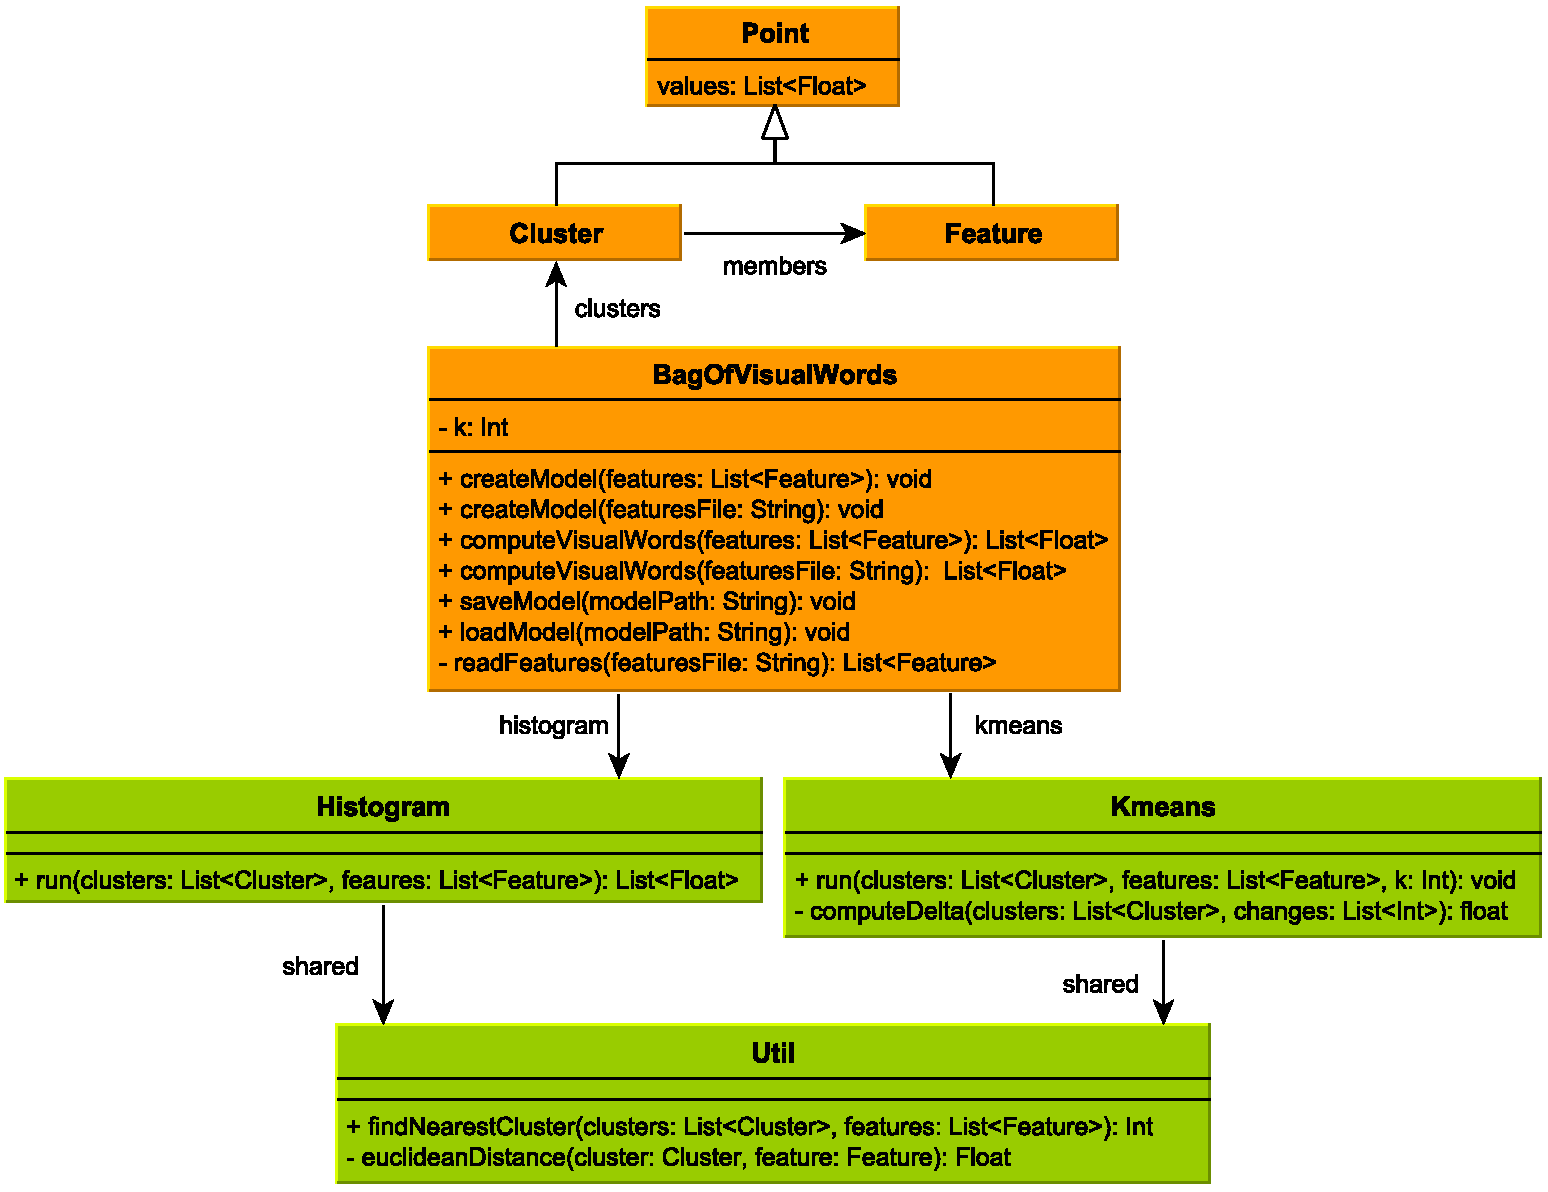
\includegraphics[scale=0.57]{images/bovw_class.pdf}
	\caption{Klassendiagramm des Bag of Visual Words}
	\label{img:bovw_class}
\end{figure}
 
\subsubsection{Generierung des Modells}

Die Generierung eines Modells kann durch die Funktion \textit{createModel} gestartet werden. Die Funktion ist überladen und erwartet als Parameter entweder eine Liste der Features oder den Pfad zu einer Datei, in der die Features gespeichert sind. Der Ablauf der Methodenaufrufe ist dann wie folgt:

\begin{itemize}
	\item Es werden bei Aufruf mit einem String die Features eingelesen und anschließend \textit{createModel} mit dieser Feature-Liste aufgerufen. Der k-means-Algorithmus wird mit den Features und \textit{k} aufgerufen. Die Daten werden zum \textit{device} kopiert und der Prozess gestartet. 
	\item Kmeans nutzt die ausgelagerte Funktion \textit{findNearestCluster} um den nächsten Cluster eines jeden Features zu bestimmen. Intern wird hier durch \textit{computeEuclideanDistance} die Entfernung eines Cluster-Feature-Paares bestimmt.
	\item Anschließend prüft \textit{computeDelta} ob sich die Zuordnung von Features zu Clustern nicht mehr wesentlich geändert hat, d.h. die relative Veränderung unter dem Schwellwert liegt.
	\item Ist der Schwellwert oder eine maximale Anzahl an Iterationen erreicht, ist der Prozess abgeschlossen und die \textit{device} Cluster werden in die Cluster des aufrufenden BagOfVisualWords-Objektes kopiert.
\end{itemize}
 
\subsubsection{Speichern und Laden eines Modells}

Um Modelle über den Speicher hinaus verwenden zu können, soll die Funktion angeboten werden, diese persistent zu speichern und wieder einlesen zu können. Die Methode \textit{saveModel(modelPath: String)} der BagOfVisualWords-Klasse speichert die Anzahl der Cluster \textit{k}, die Liste der Cluster \textit{clusters} sowie die Zuordnung der Features \textit{members} unter dem Pfad \textit{modelPath}. Durch das Pendant \textit{readModel(modelPath: String)} kann ein so gespeichertes Modell, also \textit{k}, \textit{clusters} und \textit{members}, wieder eingelesen werden.\newline
So ergibt sich zum Beispiel für ein $k = 5$ und 100 Features mit je 128 Komponenten, eine Datei mit 106 Zeilen: Die erste Zeile enthält \textit{k}. Darauf folgen \textit{k} viele, also hier fünf, Zeilen mit den Zentren der Cluster und anschließend 100 Zeilen mit den Features. Die Zeilen mit den Clustern enthalten hier 128 Werte, durch Leerzeichen separiert. Die Features enthalten einen Wert am Ende der Zeile mehr: Diese Ganzzahl gibt den Index des Clusters an, zu der das Feature gehört.

\subsubsection{Berechnung der Visual Words}

Die Erzeugung der \textit{Visual Words} wird durch die BagOfVisualWords-Klasse angestoßen. Wie bei der Modellgenerierung wird intern ein CUDA-Programm, die Histogram-Klasse, verwendet. Für den Gebrauch muss die \textit{computeVisualWords} Methode aufgerufen werden. Der Ablauf ist dann wie folgt:

\begin{itemize}
	\item Wie beim kmeans Algorithmus kann \textit{computeVisualWords} der BagOfVisualWords-Klasse mit einer Liste der Features oder dem Pfad zu einer Feature-Datei aufgerufen werden. Letztere ließt die Features ein und ruft dann wiederum \textit{computeVisualWords} mit der Feature-Liste auf. Es wird geprüft, ob ein Modell vorhanden ist, also eine Liste von Clustern vorliegt. Ist dies nicht der Fall, wird abgebrochen.
	\item Die \textit{run} Methode der Histogram-Klasse wird nun mit den \textit{clustern} der aufrufenden BagOfVisualWords-Instanz und den Features aus dem vorigen Schritt aufgerufen. Um das \textit{Visual Word} für ein Feature zu bestimmen, wird \textit{findNearestCluster} aus der Shared-Klasse genutzt. Da diese Funktion den Index des Clusters zurückgibt, kann dieser direkt für die zu inkrementierende Position im Histogramm verwendet werden.
	\item Das Histogramm wird zum \textit{host} kopiert und an den Aufrufer zurückgegeben. Es kann nun gespeichert oder für weitere Analyse verwendet werden.
\end{itemize}